\documentclass[fontset=none]{Notes}

\makeatletter
\DeclareRobustCommand{\em}{%
  \@nomath\em \if b\expandafter\@car\f@series\@nil
  \normalfont \else \bfseries \fi}
\makeatother

\usepackage{tikz-cd,wrapstuff}
\usepackage{siunitx,tikz,nicematrix}
\usetikzlibrary{matrix,calc}
\usetikzlibrary{intersections}
\usetikzlibrary{arrows.meta}

\ProvidesFile{font.def}

\setCJKmainfont{Source Han Serif SC}[
  UprightFont=*-Regular,
  BoldFont=*-Bold,
  ItalicFont=HYKaiTi S,
  ItalicFeatures={Scale=1.1}
]
\newCJKfontfamily[zhsong]\songti{Source Han Serif SC}[
  UprightFont=*-Regular,
  BoldFont=*-Bold,
  ItalicFont=HYKaiTi S,
  ItalicFeatures={Scale=1.1}
]
\setCJKsansfont{Source Han Sans SC}[
  UprightFont=*-Regular,
  BoldFont=*-Bold
]
\newCJKfontfamily[zhhei]\heiti{Source Han Sans SC}[
  UprightFont=*-Regular,
  BoldFont=*-Bold
]
\setCJKmonofont{HYFangSong S}[
  BoldFont=*,
  ItalicFont=*,
  BoldItalicFont=*
]
\newCJKfontfamily[zhfs]\fangsong{HYFangSong S}[
  BoldFont=*,
  ItalicFont=*,
  BoldItalicFont=*
]
\newCJKfontfamily[zhkai]\kaishu{HYKaiTi S}[
  BoldFont=*,
  ItalicFont=*,
  BoldItalicFont=*
]

\setmainfont{texgyretermes}[
  Extension=.otf,
  UprightFont=*-regular,
  BoldFont=*-bold,
  ItalicFont=*-italic,
  BoldItalicFont=*-bolditalic,
  SlantedFont=*-italic
]
%\setmathrm{texgyretermes}[
%  Extension=.otf,
%  UprightFont=*-regular,
%  BoldFont=*-bold,
%  ItalicFont=*-italic,
%  BoldItalicFont=*-bolditalic,
%  SlantedFont=*-italic
%]
\setsansfont{Cantarell}[
  UprightFont=* Regular,
  ItalicFont=* Italic,
  BoldFont=* Bold,
  BoldItalicFont=* Bold Italic,
  SmallCapsFont=Alegreya Sans SC
]
\setmonofont{Ubuntu Mono}[
  UprightFont=*,
  ItalicFont=* Italic,
  BoldFont=* Bold,
  BoldItalicFont=* Bold Italic
]
%\setmathfont{texgyretermes-math.otf}
%\setmathfont[range={\mathcal,\mathbfcal,\mathfrak},StylisticSet=1]{XITSMath-Regular.otf}
%\setmathfont[range={\mathbb}]{KpMath-Sans.otf}



\usepackage[subscriptcorrection,nofontinfo,mtpbb,mtpfrak]{mtpro2}
\usepackage[normal]{fixdif}

\tikzcdset{
  arrow style=tikz,
  diagrams={>={Straight Barb[scale=0.8]}}
}

\tikzset{
  every picture/.style={
    thick,
    >={Latex[width=6pt, length=8pt]}
  },
  point/.style={
    circle, fill, minimum width=5pt,
    inner sep=0pt
  }
}

\allowdisplaybreaks[1]

\newlength{\mymathln}
\newcommand{\aligninside}[2]{
  \settowidth{\mymathln}{#2}
  \mathmakebox[\mymathln]{#1}
}

\DeclareMathOperator\Spec{Spec}
\DeclareMathOperator\im{im}
\DeclareMathOperator\sgn{sgn}
\DeclareMathOperator\rad{rad}
\DeclareMathOperator\Alt{Alt}
\DeclareMathOperator\Max{Max}
\DeclareMathOperator\GL{GL}
\DeclareMathOperator\Orth{O}
\DeclareMathOperator\SO{SO}
\DeclareMathOperator\SU{SU}
\DeclareMathOperator\Lie{Lie}
\DeclareMathOperator\End{End}
\DeclareMathOperator\Int{Int}
\DeclareMathOperator\Sym{Sym}
\DeclareMathOperator\tr{tr}
\DeclareMathOperator\Hom{Hom}
\DeclareMathOperator\supp{supp}
\DeclareMathOperator\Id{Id}
\DeclareMathOperator\rk{rank}
\DeclareMathOperator\grad{grad}
\DeclareMathOperator\Euc{E}
\DeclareMathOperator\ob{ob}
\newcommand{\LL}{{\mathrm{L}}}

\newcommand{\norm}[1]{\lVert#1\rVert}
\newcommand{\mat}[1]{\mathbold{#1}}
\newcommand{\cat}[1]{\mathsf{#1}}
\newcommand{\uline}{\underline{\hphantom{X}}}
\newcommand{\abs}[1]{\left|#1\right|}
\newcommand{\lie}[1]{\mathfrak{#1}}
\newcommand{\inn}[1]{\left\langle #1\right\rangle}

\usepackage{enumitem}

\setlist[enumerate]{nosep}

%\DeclareMathAlphabet\mathcal{OMS}{cmsy}{m}{n}

\newlength\stextwidth
\newcommand\makesamewidth[3][c]{%
  \settowidth{\stextwidth}{#2}%
  \makebox[\stextwidth][#1]{#3}%
}



\begin{document}

\frontmatter

\tableofcontents

\mainmatter

\setcounter{chapter}{-1}

\chapter{导论}

\section{Brouwer 不动点定理}

我们首先概述 Brouwer 不动点定理的证明:如果 $f:D^n\to D^n$ 是连续映射,
那么存在 $x\in D^n$ 使得 $f(x)=x$。当 $n=1$ 的时候,这个定理是容易证明的,
此时 $D^1$ 是闭区间 $[-1,1]$,我们在正方形 $D^1\times D^1$ 内观察
$f$ 的图像。
\begin{figure}[h]
  \centering
  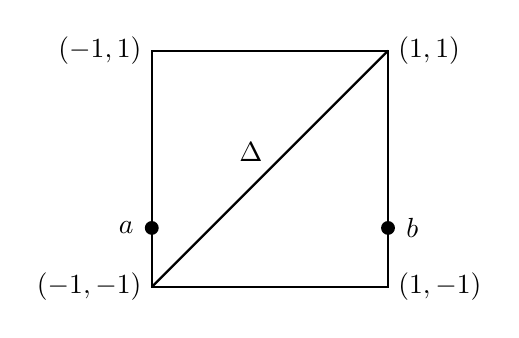
\begin{tikzpicture}[
      scale=1.5
    ]
    \draw (-1,-1) coordinate (v1) rectangle (1,1) coordinate (v2);
    \draw (v1) -- node[midway,above left=-1pt] {$\Delta$} (v2);
    \node [point,label=180:$a$] at ([yshift=0.5cm]v1) {};
    \node [point,label=0:$b$] at ([yshift=0.5cm]v1-|v2) {};
    \node [left] at (v1) {$(-1,-1)$};
    \node [left] at (v1|-v2) {$(-1,1)$};
    \node [right] at (v2) {$(1,1)$};
    \node [right] at (v2|-v1) {$(1,-1)$};
  \end{tikzpicture}
\end{figure}

\begin{theorem}
  每个连续映射 $f:D^1\to D^1$ 都有一个不动点。
\end{theorem}
\begin{proof}
  设 $f(-1)=a$ 以及 $f(1)=b$。要是 $f(-1)=-1$ 或者 $f(1)=1$,那么
  这就已经存在不动点,所以我们假设 $f(-1)=a>-1$ 以及 $f(1)=b<1$。
  设 $G$ 是 $f$ 的图像,$\Delta$ 是恒等映射的图像(对角线),我们需要证明
  $G\cap\Delta\neq \emptyset$。想法是利用连通性说明 $D^1\times D^1$
  中从 $a$ 到 $b$ 的道路必须与 $\Delta$ 相交。$f$ 连续表明 
  $G=\{(x,f(x))\,|\, x\in D^1\}$ 是连通的。定义 $A=\{(x,f(x))\,|\, f(x)>x\}$
  和 $B=\{(x,f(x))\,|\, f(x)<x\}$,注意到 $a\in A$ 和 $b\in B$。
  假设 $G\cap \Delta=\emptyset$,那么这表明 $G=A\cup B$ 是无交并,而
  $A,B$ 都是 $G$ 中的非空开集,与 $G$ 连通矛盾。
\end{proof}

不幸的是,当 $n>1$ 的时候没有人知道如何应用这个初等的拓扑证明,所以
必须引入新的思想。通过代数拓扑可以给出 Brouwer 不动点定理的一个证明。
我们最终将证明,对于每个 $n\geq 0$,存在一个\emph{同调函子} $H_n$
使得:对于每个拓扑空间 $X$,都给出一个交换群 $H_n(X)$;
对于每个连续映射 $f:X\to Y$,都给出一个同态 $H_n(f):H_n(X)\to H_n(Y)$
使得
\begin{equation}
  H_n(g\circ f)=H_n(g)\circ H_n(f)
\end{equation}
以及 $H_n(1_X)$ 是 $H_n(X)$ 上的恒等映射;此外还有
\begin{alignat}{2}
  &H_n(D^{n+1})=0 &\quad &\text{for all $n\geq 1$},\\
  &H_n(\mathbb{S}^{n})\neq 0 &&\text{for all $n\geq 1$}
  \label{eq:H_n(S^n)}.
\end{alignat}
使用 $H_n$ 的这些性质,我们现在可以证明 Brouwer 不动点定理。

\begin{definition}
  拓扑空间 $Y$ 的一个子空间 $X$ 被称为 $Y$ 的一个\emph{收缩},如果
  存在连续映射 $r:Y\to X$ 使得对于所有的 $x\in X$ 有 $r(x)=x$。
  这样的 $r$ 被称为一个\emph{收缩映射}。
\end{definition}

\begin{remark}
  (1)
  我们可以使用映射的语言重新叙述收缩映射的定义。如果 $\iota:X\hookrightarrow Y$
  是包含映射,那么连续映射 $r:Y\to X$ 是收缩映射当且仅当 $\iota$ 是 $r$ 的右逆,
  即 $r\circ\iota=1_X$。

  (2) 对于交换群来说,可以证明 $G$ 的子群 $H$ 是 $G$ 的收缩当且仅当 
  $H$ 是 $G$ 的一个直和项,也即存在 $G$ 的子群 $K$ 使得 $G=H\oplus K$。
\end{remark}

\begin{lemma}\label{lemma:S^n is not retract of D^n+1}
  如果 $n\geq 0$,那么 $\mathbb{S}^n$ 不是 $D^{n+1}$ 的收缩。
\end{lemma}
\begin{proof}
  假设存在收缩 $r:D^{n+1}\to \mathbb{S}^n$,那么我们有交换图
  \[
    \begin{tikzcd}[column sep=1.8em]
      & D^{n+1}\arrow[dr,"r"] & \\
      \mathbb{S}^n\arrow[ur,"\iota"]\arrow[rr,"1"'] & & \mathbb{S}^n ,
    \end{tikzcd}
  \]
  利用函子 $H_n$,给出了交换群的一个交换图
  \[
    \begin{tikzcd}[column sep=1em]
      & H_n(D^{n+1})\arrow[dr,"H_n(r)"] & \\
      H_n(\mathbb{S}^n)\arrow[ur,"H_n(\iota)"]\arrow[rr,"H_n(1)"'] & & 
      H_n(\mathbb{S}^n ),
    \end{tikzcd}
  \]
  由于 $H_n(D^{n+1})=0$,所以 $H_n(1)=H_n(\iota)\circ H_n(r)=0$,但是
  $H_n(1)$ 又必须是恒等映射,所以 $H_n(\mathbb{S}^n)=0$,这
  和 \eqref{eq:H_n(S^n)} 矛盾。
\end{proof}

注意到同调函子 $H_n$ 将拓扑问题转化为了代数问题。此外,
\autoref{lemma:S^n is not retract of D^n+1} 在 $n=0$ 的时候有很简单的证明,
此时收缩 $r:D^1\to \mathbb{S}^0=\{\pm 1\}$ 将连通空间映射到不连通空间,
这是不可能的。

\begin{theorem}[Brouwer]\label{thm:Brouwer}
  如果 $f:D^n\to D^n$ 是连续映射,那么 $f$ 有一个不动点。
\end{theorem}
\begin{proof}
  假设对于所有的 $x\in D^n$ 都有 $f(x)\neq x$,此时 $x$ 和 $f(x)$
  确定了一条直线。定义 $g:D^n\to \mathbb{S}^{n-1}$ 将 $x$ 映射
  为 $f(x)$ 到 $x$ 的射线与 $\mathbb{S}^{n-1}$ 的交点。
  \begin{center}
    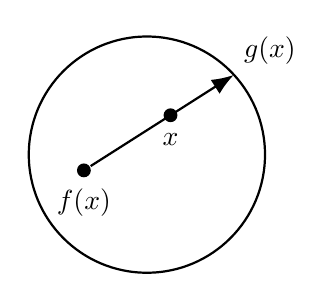
\begin{tikzpicture}
      \draw [name path=circ] (0,0) circle (1.5);
      \node [point,label=-90:$x$] (x) at (0.3,0.5) {}; 
      \node [point,label=-90:$f(x)$] (fx) at (-0.8,-0.2) {};
      \path [name path=line] (fx) -- ($(fx)!2!(x)$);
      \draw [->,name intersections={of=circ and line, by={gx}}]
        (fx) -- (gx) node [above right] {$g(x)$};
    \end{tikzpicture}
  \end{center}
  显然
  $x\in \mathbb{S}^{n-1}$ 表明 $g(x)=x$。利用坐标不难计算得 $g$ 
  是连续映射。
  这样 $g$ 就构成了一个收缩映射,与前面的引理矛盾。
\end{proof}

\begin{problem}{}{}
令 $H$ 是交换群 $G$ 的子群。如果存在同态 $r:G\to H$ 使得
对任意 $x\in H$ 有 $r(x)=x$,那么 $G=H\oplus \ker r$。  
\end{problem}
\begin{proof}
  任取 $y\in G$,那么 $r(y-r(y))=r(y)-r(y)=0$,所以
  $y-r(y)\in\ker r$,所以 $y=r(y)+y-r(y)\in H+\ker r$,
  所以 $G=H+\ker r$。下面设 $x\in H\cap\ker r$,那么
  $x=r(x)=0$,所以 $H\cap\ker r=\emptyset$。
\end{proof}

\begin{problem}{}{}
  假设在 $n\geq 1$ 的时候已知
  \[
    H_i(\mathbb{S}^n)=\begin{cases}
      \mathbb{Z} & i=0,n,\\
      0 & \text{otherwise},
    \end{cases}
  \]
  证明 $\mathbb{S}^{n}$ 的赤道不是一个收缩。
\end{problem}
\begin{proof}
  设 $r:\mathbb{S}^n\to \mathbb{S}^{n-1}$ 是收缩映射。
  那么我们有交换图
  \[
    \begin{tikzcd}[column sep=1em]
      & H_i(\mathbb{S}^{n})\arrow[dr,"H_i(r)"] & \\
      H_i(\mathbb{S}^{n-1})\arrow[ur,"H_i(\iota)"]\arrow[rr,"H_i(1)"'] & & 
      H_i(\mathbb{S}^{n-1}),
    \end{tikzcd}
  \]
  取 $i=n-1$ 即可得出矛盾。
\end{proof}

\begin{problem}{}{}
  如果 $X$ 是同胚于 $D^n$ 的拓扑空间,那么连续映射
  $f:X\to X$ 有不动点。
\end{problem} 
\begin{proof}
  设 $\varphi:D^n\to X$ 是同胚映射,那么 $\varphi^{-1}\circ f\circ\varphi:D^n\to D^n$
  是连续映射且有不动点,即存在 $x$ 使得 $\varphi^{-1}(f(\varphi(x)))=x$,
  即 $f(\varphi(x))=\varphi(x)$,所以 $f$ 有不动点 $\varphi(x)$。
\end{proof}

\begin{problem}{}{}
  令 $f,g:I\to I\times I$ 是连续映射,并且 $f(0)=(a,0)$,
  $f(1)=(b,1)$,$g(0)=(0,c)$,$g(1)=(1,d)$。证明存在 $s,t\in I$
  使得 $f(s)=g(t)$,也就是说 $f$ 和 $g$ 的像集一定是相交的道路。
\end{problem}
\begin{proof}
  定义 $h:I\times I\to I\times I$ 为
\end{proof}


\section{范畴与函子}

\begin{definition}
  范畴 $\cat C$ 上的一个\emph{共轭}指的是所有态射的类 $\bigcup_{(A,B)}\Hom(A,B)$
  上的一个等价关系 $\sim$,满足:
  \begin{enumerate}
    \item 如果 $f\in\Hom(A,B)$ 以及 $f\sim f'$,那么 $f'\in\Hom(A,B)$;
    \item 如果 $f\sim f'$ 和 $g\sim g'$ 并且 $g\circ f$ 存在,那么
    $g\circ f\sim g'\circ f'$。
  \end{enumerate}
\end{definition}

\begin{theorem}
  令 $\cat C$ 是一个范畴附带一个共轭 $\sim$,令 $[f]$ 表示态射 $f$ 的等价类。
  定义 $\cat C'$ 为:
  \begin{align*}
    \ob \cat C'&=\ob \cat C;\\
    \Hom_{\cat C'}(A,B)&=\bigl\{[f]\bigm| f\in\Hom_{\cat C}(A,B)\bigr\};\\
    [g]\circ [f]&=[g\circ f].
  \end{align*}
  那么 $\cat C'$ 是一个范畴,称为 $\cat C'$ 的\emph{商范畴}。
\end{theorem}

\chapter{基本拓扑概念}

\section{同伦}

\begin{definition}
  如果 $X,Y$ 是拓扑空间,$f_0,f_1$ 是 $X$ 到 $Y$ 的连续映射,存在
  连续映射 $F:X\times I\to Y$ 使得
  \[
    F(x,0)=f_0(x),\quad F(x,1)=f_1(x),
  \]
  那么我们说 $F$ 是一个\emph{同伦映射},并且 $f_0$ \emph{同伦于}
  $f_1$,记为 $f_0\simeq f_1$。当需要强调同伦映射的时候,我们写作
  $F:f_0\simeq f_1$。
\end{definition}

如果记 $f_t:X\to Y$ 为 $f_t(s)=F(x,t)$,那么同伦 $F$ 给出了一族
从 $f_0$ 变形到 $f_1$ 的单参数连续映射。我们可以认为 $f_t$ 随着
时间 $t$ 变形。

\begin{lemma}[粘连引理]
  假设 $X$ 是有限个闭子集的并集:$X=\bigcup_{i=1}^n X_i$。
  如果对于某个空间 $Y$,存在一族连续映射 $f_i:X_i\to Y$,它们在
  重叠区域相同,即对于任意 $i,j$ 有 $f_i|_{X_i\cap X_j}=f_j|_{X_i\cap X_j}$,
  那么存在唯一的连续映射 $f:X\to Y$ 使得对于所有的 $i$ 有 $f|_{X_i}=f_i$。
\end{lemma}
\begin{proof}
  任取 $x\in X$,如果 $x\in X_i$,我们定义 $f(x)=f_i(x)$。
  由于 $f_i,f_j$ 在重叠区域相同,所以这个定义是良好的,我们只需要说明连续性。
  任取 $Y$ 的闭子集 $C$,那么
  \begin{equation*}
    f^{-1}(C)=\bigcup\bigl(X_i\cap f^{-1}(C)\bigr)=
    \bigcup f_i^{-1}(C),
  \end{equation*}
  由于 $f_i^{-1}(C)$ 是 $X_i$ 的闭集,所以是 $X$ 的闭集。
  所以 $f^{-1}(C)$ 是闭集,即 $f$ 是连续映射。
\end{proof}

粘合引理也可以有开集的版本,其证明是完全一致的。

\begin{lemma}{}{}
  假设 $X$ 是任意个开子集的并集:$X=\bigcup_i X_i$。
  如果对于某个空间 $Y$,存在一族连续映射 $f_i:X_i\to Y$,它们在
  重叠区域相同,
  那么存在唯一的连续映射 $f:X\to Y$ 使得对于所有的 $i$ 有 $f|_{X_i}=f_i$。
\end{lemma}

\begin{theorem}
  同伦是所有连续映射 $X\to Y$ 集合上的一个等价关系。
\end{theorem}
\begin{proof}
  \emph{自反性}。如果 $f:X\to Y$ 是连续映射,定义 $F(x,t)=f(x)$,
  显然 $F:f\simeq f$。

  \emph{对称性}。假设 $f\simeq g$,即存在连续映射 $F:X\times I\to Y$
  使得 $F(x,0)=f(x)$ 和 $F(x,1)=g(x)$。定义 $G:X\times I\to Y$
  为 $G(x,t)=F(x,1-t)$,那么 $G:g\simeq f$。

  \emph{传递性}。假设 $F:f\simeq g$ 以及 $G:g\simeq h$。定义
  $H:X\times I\to Y$ 为
  \[
    H(x,t)=\begin{cases}
      F(x,2t) & 0\leq t\leq \frac{1}{2},\\
      G(x,2t-1) & \frac{1}{2}\leq t\leq 1.
    \end{cases}
  \]
  根据粘合引理,所以 $H$ 连续,所以 $H:f\simeq h$。
\end{proof}

\begin{definition}
  如果 $f:X\to Y$ 是连续映射,我们说
  \[
    [f]=\{g:X\to Y\,|\, g\simeq f\}
  \]
  是 $f$ 的\emph{同伦类}。
\end{definition}

所有同伦类的集合记为 $[X,Y]$。

\begin{theorem}
  对于 $i=0,1$,令 $f_i:X\to Y$ 和 $g_i:Y\to Z$ 是连续映射。如果
  $f_0\simeq f_1$ 和 $g_0\simeq g_1$,那么 $g_0\circ f_0\simeq g_1\circ f_1$,
  即 $[g_0\circ f_0]=[g_1\circ f_1]$。
\end{theorem}
\begin{proof}
  令 $F:f_0\simeq f_1$ 和 $G:g_0\simeq g_1$ 是同伦映射。
  首先定义 $H:X\times I\to Z$ 为 $H(x,t)=G(f_0(x),t)$,
  那么 $H:g_0\circ f_0\simeq g_1\circ f_0$。
  另一方面,定义 $K:X\times I\to Z$ 为 $K(x,t)=g_1\circ F(x,t)$,
  那么 $K:g_1\circ f_0\simeq g_1\circ f_1$。
  根据同伦的传递性,就有 $g_1\circ f_1\simeq g_0\circ f_0$。
\end{proof}

\begin{corollary}
  同伦是拓扑范畴 $\cat{Top}$ 上的一个共轭。
\end{corollary}

这意味着存在一个商范畴,其对象是拓扑空间 $X$,态射集合 
$\Hom(X,Y)=[X,Y]$,复合为 $[g]\circ [f]=[g\circ f]$。

\begin{definition}
  上述商范畴被称为\emph{同伦范畴},记为 $\cat{hTop}$。
\end{definition}

我们即将构造的所有从 $\cat{Top}$ 到某个“代数”范畴 $\cat A$(例如 $\cat{Ab},\cat{Grp},\cat{Ring}$)
的函子 $T:\cat{Top}\to\cat{A}$ 都有性质使得 $f\simeq g$ 的时候有 $T(f)=T(g)$。
事实上,除开自然地希望将同伦映射视为等同的之外,这保证了通过 $T$
将拓扑问题转化为 $\cat A$ 中的代数问题是比原问题更加简单的。
此外,练习表明每个这样的函子都会给出一个函子 $\cat{hTop}\to\cat A$,
所以同伦范畴是相当基本的。

\begin{definition}
  一个连续映射 $f:X\to Y$ 被称为\emph{同伦等价},如果存在连续映射
  $g:Y\to X$ 使得 $g\circ f\simeq 1_X$ 和 $f\circ g\simeq 1_Y$。
  如果存在同伦等价 $f:X\to Y$,那么我们说空间 $X$ 和 $Y$
  有相同的\emph{同伦型}。
\end{definition}

显然,同胚的空间有相同的同伦型,但是反过来不对,我们将在后面看到。

下面的两个结果表明同伦可以和一些有趣的问题联系起来。

\begin{definition}
  令 $X,Y$ 是拓扑空间,$y_0\in Y$。$y_0$ 处的\emph{常值映射}
  指的是映射 $c:X\to Y$ 使得 $c(x)\equiv y_0$。
  对于连续映射 $f:X\to Y$,如果存在常值映射 $c$ 使得 $f\simeq c$,那么我们说 $f$ 是
  \emph{零伦的}。
\end{definition}

\begin{remark}
  我们将在后面看到 $\mathbb{C}\smallsetminus\{0\}$ 实质上是圆周
  $\mathbb{S}^1$,即 $\mathbb{C}\smallsetminus\{0\}$ 和 $\mathbb{S}^1$
  有相同的同伦型。
\end{remark}

拓扑学中一个常见的问题是将映射 $f:X\to Z$ 延拓到一个更大的空间 $Y$
中,即是否存在 $g:Y\to Z$ 使得有下面的交换图
\[
  \begin{tikzcd}[column sep=large,row sep=large]
    Y\arrow[dr,"g",dashrightarrow] & \\
    X\arrow[u,hook]\arrow[r,"f"'] & Z  .
  \end{tikzcd}
\]
同伦本身则引出了这样一个问题:如果 $f_0,f_1:X\to Z$ 且我们能够
延拓 $f_0\cup f_1:X\times\{0\}\cup X\times\{1\}\to Z$ 到
$X\times I$ 上,那么 $f_0\simeq f_1$。

\begin{theorem}
  令 $f:\mathbb{S}^n\to Y$ 是连续映射,下面的说法等价:
  \begin{enumerate}
    \item $f$ 是零伦的;
    \item $f$ 可以延拓为一个连续映射 $D^{n+1}\to Y$;
    \item 如果 $x_0\in \mathbb{S}^n$,$k:\mathbb{S}^n\to Y$
    是 $f(x_0)$ 处的常值映射,那么存在一个同伦 $F:f\simeq k$
    使得 $F(x_0,t)=f(x_0)$ 对于所有 $t\in I$ 成立。
  \end{enumerate}
\end{theorem}
\begin{proof}
  $(1)\Rightarrow(2)$ 假设 $F:f\simeq c$,其中 $c(x)=y_0$。定义
  $g:D^{n+1}\to Y$ 为
  \[
    g(x)=\begin{cases}
      y_0 & 0\leq \norm{x}\leq\frac{1}{2},\\
      F\bigl(x/\norm{x},2-2\norm{x}\bigr) & 
      \frac{1}{2}\leq\norm{x}\leq 1.
    \end{cases}
  \]
  根据粘合引理,$g$ 是连续映射。如果 $x\in \mathbb{S}^n$,那么
  $g(x)=F(x,0)=f(x)$,所以 $g$ 是 $f$ 的延拓。

  $(2)\Rightarrow(3)$ 假设 $g:D^{n+1}\to Y$ 是 $f$ 的延拓。定义
  $F:\mathbb{S}^{n}\times I\to Y$ 为 $F(x,t)=g((1-t)x+tx_0)$,
  显然 $F$ 是连续映射。由于 $F(x,0)=g(x)=f(x)$,$F(x,1)=g(x_0)=f(x_0)$,
  所以 $F:f\simeq k$。此外,$F(x_0,t)=g(x_0)=f(x_0)$。

  $(3)\Rightarrow (1)$ 显然。
\end{proof}

我们可以把这个定理和 \autoref{lemma:S^n is not retract of D^n+1} 对比。
如果 $Y=\mathbb{S}^n$ 以及 $f$ 是恒等映射,那么 \autoref{lemma:S^n is not retract of D^n+1}
表明 $f$ 不是零伦的,否则 $f$ 延拓为连续映射 $D^{n+1}\to \mathbb{S}^n$,这表明
$\mathbb{S}^n$ 是 $D^{n+1}$ 的收缩。

\section{凸性、可缩性以及锥体}

我们给上述证明中使用到的 $D^{n+1}$ 的一个性质起个名字。

\begin{definition}
  $\mathbb{R}^m$ 的子集 $X$ 被称为\emph{凸集},如果任取 $x,y\in X$,
  连接 $x,y$ 的线段都在 $X$ 中。换句话说,对于任意 $t\in I$,有
  $tx+(1-t)y\in X$。
\end{definition}

凸集的例子有很多,例如 $I^n$,$\mathbb{R}^n$,$D^n$ 和 $\Delta^n$
都是凸集。但是球面 $\mathbb{S}^n\subseteq \mathbb{R}^{n+1}$
不是凸集。

\begin{definition}
  空间 $X$ 被称为\emph{可缩的},如果 $1_X$ 是零伦的。
\end{definition}

\begin{theorem}
  每个凸集 $X$ 都是可缩的。
\end{theorem}
\begin{proof}
  任取 $x_0\in X$,定义 $c:X\to X$ 是常值映射 $c(x)=x_0$。
  令 $F:X\times I\to X$ 为 $F(x,t)=tx_0+(1-t)x$,那么 $F:1_X\simeq c$。
\end{proof}

半球面是可缩的但是不是凸集,所以上述定理的逆命题不正确。后面我们会
发现 \autoref{lemma:S^n is not retract of D^n+1} 实际上表明
$\mathbb{S}^n$ 是不可缩的。

\begin{problem}{}{}
  (1) 如果 $X\approx Y$ 且 $X$ 可缩,那么 $Y$ 也可缩。

  (2) 如果 $X,Y$ 是 Euclid 空间的子空间,$X\approx Y$ 且 $X$
  是凸集,证明 $Y$ 可能不是凸集。 
\end{problem}
\begin{proof}
  (1) 设 $c:X\to X$ 是常值映射 $c(x)=x_0$ 且 $1_X\simeq c$,
  $f:X\to Y$ 是同伦等价。设 $g:Y\to X$
  使得 $g\circ f\simeq 1_X$ 以及 $f\circ g\simeq 1_Y$。
  记 $k:Y\to Y$ 是常值映射 $k(y)=f(x_0)$,那么
  \[
    1_Y=1_Y \circ 1_Y\simeq 
    (f\circ g)\circ (f\circ g)\simeq f\circ 1_X\circ g
    \simeq f\circ c\circ g=k,
  \]
  所以 $Y$ 可缩。
\end{proof}

\begin{problem}{}{}
  令 $R:\mathbb{S}^1\to \mathbb{S}^1$ 表示旋转 $\alpha$ 弧度。证明
  $R\simeq 1_{\mathbb{S}^1}$。由此得出每个连续映射 $f:\mathbb{S}^1\to \mathbb{S}^1$
  都同伦于一个满足 $g(1)=1$ 的连续映射 $g:\mathbb{S}^1\to \mathbb{S}^1$。
\end{problem}
\begin{proof}
  即 $R(e^{i\theta})=e^{i(\theta+\alpha)}$。定义 $F:\mathbb{S}^1\times I\to \mathbb{S}^1$
  为 $F(e^{i\theta},t)=e^{i(\theta+t\alpha)}$,显然 $F$ 是连续映射,
  所以 $F:1_{\mathbb{S}^1}\simeq R$。任取连续映射 $f:\mathbb{S}^1\to \mathbb{S}^1$,
  设 $f(1)=e^{i\alpha}$,取 $R$ 为旋转 $-\alpha$,
  那么 $1_{\mathbb{S}^1}\circ f\simeq R\circ f$,此时 $g=R\circ f$
  满足 $g(1)=R(f(1))=1$。
\end{proof}

马上引入的锥体的构造将表明每个空间都可以嵌入到一个可缩空间中。
我们先回顾一下商空间的构造。

\begin{definition}
  令 $X$ 是拓扑空间,$\sim$ 是一个等价关系,那么有一个自然映射
  $\pi:X\to X/\sim$,即 $\pi(x)=[x]$。我们可以赋予 $X/\sim$ 一个\emph{商拓扑},
  即 $U\subseteq X/\sim$ 是开集当且仅当 $\pi^{-1}(U)$ 是 $X$
  的开集。
\end{definition}

有一种特殊的情况需要单独提及。如果 $A\subseteq X$,那么我们记 $X/A$
为划分 $\{A\}\cup \{\{x\}\,|\, x\in X \smallsetminus A\}$ 给出的商空间,
也就是说,这个构造将 $A$ 压缩为一点,而 $X \smallsetminus A$ 中的点保持不变。

\begin{definition}
  连续满射 $f:X\to Y$ 被称为\emph{商映射},如果 $U\subseteq Y$
  是开集当且仅当 $f^{-1}(U)$ 是 $X$ 的开集。
\end{definition}

\begin{example}
  \mbox{}
  \begin{enumerate}
    \item 自然映射 $\pi:X\to X/\sim$ 是商映射。
    \item 如果连续满射 $f:X\to Y$ 是开映射或者闭映射,那么 $f$
    是商映射。以开映射的情况为例,此时若 $U\subseteq Y$ 使得 $f^{-1}(U)$
    是开集,那么 $U=f(f^{-1}(U))$ 是 $Y$ 的开集。
    \item 如果连续映射 $f:X\to Y$ 有一个截面,即存在连续映射 $s:Y\to X$
    使得 $f\circ s=1_Y$,那么 $f$ 是商映射。首先 $s$ 是 $f$ 是右逆保证了
    $f$ 是满射。若 $U\subseteq Y$ 使得 $f^{-1}(U)$ 是开集,那么 
    $U=1_Y^{-1}(U)=(f\circ s)^{-1}(U)$ 是 $Y$ 的开集,所以 $f$
    是商映射。
  \end{enumerate}
\end{example}

\begin{theorem}
  令 $f:X\to Y$ 是连续满射。那么 $f$ 是商映射当且仅当:对于 
  任意空间 $Z$ 和映射 $g:Y\to Z$,$g$ 连续当且仅当 $g\circ f$ 连续。
  \[
    \begin{tikzcd}[column sep=large,row sep=large]
      X\arrow[d,"f"']\arrow[dr,"g\circ f"] & \\
      Y\arrow[r,"g"'] & Z.
    \end{tikzcd}
  \]
\end{theorem}
\begin{proof}
  假设 $f$ 是商映射。如果 $g$ 连续,显然 $g\circ f$ 连续。反之,如果
  $g\circ f$ 连续,任取 $Z$ 的开集 $V$,那么 
  $f^{-1}(g^{-1}(V))=(g\circ f)^{-1}(V)$ 是 $X$ 的开集,所以
  $g^{-1}(V)$ 是 $Y$ 的开集,所以 $g$ 连续。

  假设反过来成立。取 $Z=X/\sim$,$\sim$ 是映射 $f$ 的纤维诱导的 
  $X$ 的划分。那么我们有交换图
  \[
    \begin{tikzcd}[sep=large]
      X\arrow[d,"f"']\arrow[dr,"\pi"] &  \\
      Y & X/\sim\arrow[l,"\bar f"],
    \end{tikzcd}
  \]
  其中 $\bar f$ 是 $f$ 诱导的双射,此时 $\bar f^{-1}\circ f(x)=\pi(x)$,
  根据假设,$\bar f^{-1}$ 是连续映射,所以 $\bar f$ 是同胚,所以
  $f=\bar f\circ\pi$ 是商映射。
\end{proof}

\begin{corollary}
  令 $f:X\to Y$ 是商映射,$h:X\to Z$ 是连续映射并且在 $f$
  的每个纤维上是常值的,那么存在唯一的连续映射 $\bar h:Y\to Z$
  使得 $h=\bar h\circ f$,即有交换图
  \[
    \begin{tikzcd}[sep=large]
      X\arrow[d,"f"']\arrow[dr,"h"] &  \\
      Y\arrow[r,"\bar h"',dashed] & Z.
    \end{tikzcd}
  \]
  此外,$\bar h$ 是开(闭)映射当且仅当在
  $U$ 是 $X$ 的形如 $U=f^{-1}(f(U))$ 的开(闭)集时,
  $h(U)$ 是 $Z$ 的开(闭)集。
\end{corollary}
\begin{proof}
  要保证 $h=\bar h\circ f$,即任取 $x\in X$,有 $\bar h(f(x))=h(x)$。
  对于 $y=f(x)\in Y$,那么必须有 $\bar h(y)=\bar h(f(x))=h(x)$,
  $h$ 在 $f$ 的纤维上是常值的表明这样的 $\bar h$ 是良好定义的,所以
  $\bar h$ 唯一存在。$h=\bar h\circ f$ 连续表明 $\bar h$ 连续。

  以开映射为例。若 $\bar h$ 是开映射且 $U=f^{-1}(f(U))$ 是
  $X$ 的开集,那么 $h(U)=h(f^{-1}(f(U)))=\bar h(f(U))$,
  由于 $f^{-1}(f(U))=U$ 是 $X$ 的开集,所以 $f(U)$ 是 $Y$
  的开集,所以 $h(U)=\bar h(f(U))$ 是 $Z$ 的开集。
  反之,任取 $V\subseteq Y$ 是开集,那么 $f^{-1}(V)$ 是 $X$
  的开集且 $f^{-1}(V)=f^{-1}(f(f^{-1}(V)))$,
  根据假设,有 $h(f^{-1}(V))$ 是 $Z$ 的开集,
  于是 $\bar h(V)=\bar h(f(f^{-1}(V)))=h(f^{-1}(V))$
  是 $Z$ 的开集,即 $\bar h$ 是开映射。
\end{proof}

\begin{corollary}
  令 $X,Z$ 是拓扑空间,$h:X\to Z$ 是商映射,记 $X/\sim$ 是 $h$ 的纤维
  导出的商空间,那么 $X/\sim$ 同胚于 $Z$,同胚映射为 $\varphi:[x]\mapsto h(x)$。
\end{corollary}
\begin{proof}
  记自然映射 $\pi:X\to X/\sim$。由于 $h$ 在 $h$ 的纤维上是常值的,
  所以存在唯一的连续映射 $\varphi:X/\sim\,\to Z$ 使得 $h=\varphi\circ\pi$,
  即 $\varphi([x])=h(x)$。另一方面,$\pi$ 在 $h$ 的纤维上也是常值的,所以
  存在唯一的连续映射 $\psi:Z\to X/\sim$ 使得 $\pi=\psi\circ h$,
  所以 $h=\varphi\circ\pi=\varphi\circ\psi\circ h$,$h$
  是满射表明存在右逆,所以 $\varphi\circ\psi=1_Z$。
  同理可得 $\psi\circ\varphi=1_{X/\sim}$,所以 $\varphi$
  和 $\psi$ 互为连续逆映射,故 $\varphi$ 是同胚。
\end{proof}

\begin{problem}{}{}
  令 $f:X\to Y$ 是商映射,$g:Y\to Z$ 是连续满射,那么 $g$
  是商映射当且仅当 $g\circ f$ 是商映射。 
\end{problem}
\begin{proof}
  若 $g$ 是商映射,设 $W\in Z$ 使得 $(g\circ f)^{-1}(W)$
  是 $X$ 的开集,即 $f^{-1}(g^{-1}(W))$ 是 $X$ 的开集,
  所以 $g^{-1}(W)$ 是 $Y$ 的开集,所以 $W$ 是 $Z$
  的开集,所以 $g\circ f$ 是商映射。

  反之,若 $g\circ f$ 是商映射。设 $W\in Z$ 使得 $g^{-1}(W)$
  是开集,那么 $(g\circ f)^{-1}(W)=f^{-1}(g^{-1}(W))$
  是 $X$ 的开集,$g\circ f$ 是商映射表明 $W$ 是 $Z$ 的开集。
\end{proof}

\begin{problem}{}{}
  设 $X$ 和 $Y$ 是拓扑空间,分别有等价关系 $\sim$ 和 $\sim'$,
  $f:X\to Y$ 是保持关系的连续映射,即 $x\sim x'$ 能推出 $f(x)\sim' f(x')$。
  证明其诱导的 $\bar f:X/\sim\,\to Y/\sim'$ 是连续映射。此外,
  如果 $f$ 是商映射,那么 $\bar f$ 也是商映射。
\end{problem}
\begin{proof}
  记 $\pi:X\to X/\sim$ 和 $\pi':Y\to Y/\sim'$ 是自然映射。
  那么我们有交换图
  \[
    \begin{tikzcd}[sep=huge]
      X\arrow[r,"f"]\arrow[d,"\pi"'] & Y\arrow[d,"\pi'"]\\
      X/\sim\arrow[r,"\bar f"',dashed] & Y/\sim',
    \end{tikzcd}
  \] 
  其中 $\bar f([x])=[f(x)]$。$f$ 保持关系表明 $\bar f$ 是良好定义的。
  任取 $Y/\sim'$ 的开集 $V$,那么 
  \[
    \pi^{-1}(\bar f^{-1}(V))=(\bar f\circ\pi)^{-1}(V)=(\pi'\circ f)^{-1}(V)=f^{-1}(\pi'^{-1}(V))
  \]
  是 $X$ 的开集,所以 $\bar f^{-1}(V)$ 是 $X/\sim$ 的开集,
  故 $\bar f$ 是连续映射。如果 $f$ 是商映射,那么
  $\pi'\circ f$ 是商映射,再根据上一题,$\bar f$ 是商映射。
\end{proof}

\begin{definition}
  若 $X$ 是拓扑空间,定义 $X\times I$ 上的等价关系为 $(x,t)\sim (x',t')$
  当且仅当 $t=t'=1$。记 $(x,t)$ 所在的等价类为 $[x,t]$。
  我们说商空间 $X\times I/\sim$ 是 $X$ 上的\emph{锥体},记为 $CX$。
\end{definition}

实际上上面的定义表明 $CX$ 就是商空间 $X\times I/X\times\{1\}$。
点 $[x,1]\in CX$ 被称为\emph{顶点}。我们基本上相当于引入了一个新的不在
$x$ 中的点(顶点)$v$ 并且用线段连接了 $v$ 和 $X$ 中的每个点。

\begin{example}
  对于空间 $X$ 和 $Y$,任意连续映射 $f:X\times I\to Y$
  如果满足 $f(x,1)=y_0$,那么都诱导了连续映射 $\bar f:CX\to Y$
  为 $\bar f:[x,t]\mapsto f(x,t)$。特别地,令 $f:\mathbb{S}^{n}\times I\to D^{n+1}$
  是映射 $(u,t)\mapsto (1-t)u$,因为 $f(u,1)\equiv 0$,所以诱导连续映射
  $\bar f:C \mathbb{S}^n\to D^{n+1}$ 为 $[u,t]\mapsto (1-t)u$。实际上,
  $\bar f$ 还是一个同胚。我们说明 $f$ 是商映射即可,由于 $f$
  是紧空间到 Hausdorff 空间的连续映射,所以是闭映射,又因为 $f$
  是满射,所以 $f$ 是商映射。
\end{example}

\begin{theorem}
  对于每个空间 $X$,锥体 $CX$ 都是可缩的。
\end{theorem}
\begin{proof}
  定义 $F:CX\times I\to CX$ 为
  $F([x,t],s)=[x,s+(1-s)t]$ 即可。
\end{proof}

下面的结果表明可缩空间是 $\cat{hTop}$ 中最简单的对象。

\begin{theorem}
  空间 $X$ 和单点空间有相同的同伦型当且仅当 $X$ 是可缩的。
\end{theorem}
\begin{proof}
  设 $\{a\}$ 是单点空间。假设 $X$ 和 $\{a\}$ 有相同的同伦型,
  即存在连续映射 $f:X\to\{a\}$ 和连续映射 $g:\{a\}\to X$
  使得 $g\circ f\simeq 1_X$,由于 $g\circ f$ 显然是常值映射,
  所以 $X$ 是可缩的。

  假设 $X$ 是可缩的。设 $1_X\simeq c$,其中 $c:X\to X$ 是常值映射
  $c(x)=x_0$。令 $f:X\to \{x_0\}$ 和 $g:\{x_0\}\to X$,
  其中 $g(x_0)=x_0$。那么 $f\circ g=1_{\{x_0\}}$ 以及
  $g\circ f=c\simeq 1_X$,所以 $f:X\to \{x_0\}$ 是同伦等价。
\end{proof}

下面的定理表明可缩空间可能和单点集的行为类似,尤其是以同伦的角度来看的时候。

\begin{theorem}
  如果 $Y$ 可缩,那么任意 $X\to Y$ 的两个连续映射都是同伦的,
  等价地说,任意 $X\to Y$ 的连续映射都是零伦的。
\end{theorem}
\begin{proof}
  $Y$ 可缩表明 $1_Y\simeq c$,设 $c(y)=y_0$ 是常值映射。
  定义 $g:X\to Y$ 是常值映射 $g(x)=y_0$。任取连续映射 $f:X\to Y$,那么
  $f=1_Y\circ f\simeq c\circ f=g$,所以任意连续映射 $f$
  都同伦于 $g$。
\end{proof}
 
\section{道路和道路连通}

\begin{definition}
  $X$ 的一个\emph{道路}指的是一个连续映射 $f:I\to X$。如果 
  $f(0)=a$,$f(1)=b$,那么我们说 $f$ 是从 $a$ 到 $b$ 的道路。
\end{definition}

\begin{definition}
  如果对于任意 $a,b\in X$,都存在从 $a$ 到 $b$ 的道路,那么我们说
  $X$ 是\emph{道路连通}的。
\end{definition}

\begin{theorem}
  如果 $X$ 道路连通,那么 $X$ 连通。
\end{theorem}
\begin{proof}
  假设 $X$ 不连通,那么存在分离开集 $A,B$ 使得 $X=A\cup B$。
  取 $a\in A$ 和 $b\in B$,$X$ 道路连通表明存在从 $a$ 到 $b$
  的道路 $f:I\to X$,那么 $f(I)$ 是连通子集,但是
  $f(I)=\bigl(f(I)\cap A\bigr)\cup\bigl(f(I)\cap B\bigr)$,
  这与 $f(I)$ 连通矛盾。
\end{proof}

\begin{example}
  存在连通但是不道路连通的空间。\emph{拓扑学家的 sin 曲线}是一个
  经典的例子。定义空间 $X=A\cup G\subseteq \mathbb{R}^2$ 由两部分构成,
  其中 $A=\{(0,y)\,|\, -1\leq y\leq 1\}$,
  $G=\{(x,\sin(1/x))\,|\, 0<x\leq 1/2\pi\}$。
  不难证明 $X$ 是连通的,因为 $A\subseteq \wbar G$,
  所以 $X=\wbar G$ 是连通的。但是 $X$ 不是道路连通的。
  我们证明不存在从 $(0,0)$ 到 $(1/2\pi,0)$ 的道路。
  假设 $f:I\to X$ 是这样的道路,取 $t_0=\sup\{t\in I\,|\, f(t)\in A\}$,
  由于 $A$ 是 $X$ 的闭集,所以 $f^{-1}(A)\subseteq [0,t_0]$
  是闭集,而 $t_0$ 是 $f^{-1}(A)$ 的极限点,所以 $f(t_0)\in A$。
  同时,任意 $s\in (t_0,1]$ 都使得 $f(s)\in G$。那么我们可以选取
  递减趋于 $t_0$ 的一列 $\{s_n\}$ 使得 $f(s_n)=\bigl(2/(2n+1)\pi,(-1)^n\bigr)$,
  但是 $n\to\infty$ 的时候 $f(s_n)$ 并不收敛,这与 $f$ 的连续性矛盾。
\end{example}

\begin{problem}{}{}
  (1) 空间 $X$ 是道路连通的当且仅当任意两个常值映射
    $X\to X$ 是同伦的。

  (2) 如果 $X$ 可缩,$Y$ 道路连通,那么任意两个连续映射 $X\to Y$
  是同伦的。
\end{problem}
\begin{proof}
  (1) 若 $X$ 道路连通,$c_1,c_2$ 分别是点 $x_1,x_2$ 处的常值映射。
  设 $f:I\to X$ 是连接 $x_1,x_2$ 的道路,定义 $F:X\times I\to X$
  为 $F(x,t)=f(t)$,那么 $F:c_1\simeq c_2$。
  反之,若任意两个常值映射 $X\to Y$ 都同伦。任取 $x_1,x_2\in X$,
  那么常值映射 $c_1(x)=x_1$ 和 $c_2(x)=x_2$ 同伦,设 
  $F:c_1\simeq c_2$,那么 $f(t)=F(x_1,t)$ 就是连接 $x_1,x_2$ 的道路。

  (2) $X$ 可缩表明 $1_X\simeq c$,其中 $c$ 是常值映射 $c(x)=x_0$。
  任取连续映射 $f:X\to Y$,那么 $f=f\circ 1_X\simeq f\circ c$,
  其中 $f\circ c$ 是常值映射,所以 $f$ 零伦。$Y$ 道路连通表明任意
  $X\to Y$ 的两个常值映射同伦,所以任意两个连续映射 $X\to Y$
  是同伦的。
\end{proof}

\begin{problem}{}{}
  如果 $X,Y$ 道路连通,那么 $X\times Y$ 道路连通。
\end{problem}
\begin{proof}
  任取 $(x_1,y_1),(x_2,y_2)\in X\times Y$,存在从 $x_1$
  到 $x_2$ 的道路 $f:I\to X$ 以及从 $y_1$ 到 $y_2$ 的道路
  $g:I\to Y$,令 $h:I\to X\times Y$ 为 $h(t)=(f(t),g(t))$,
  那么 $h$ 为从 $(x_1,y_1)$ 到 $(x_2,y_2)$ 的道路。
\end{proof}

\begin{problem}{}{}
  若 $f:X\to Y$ 是连续映射且 $X$ 道路连通,那么 $f(X)$ 道路连通。
\end{problem}
\begin{proof}
  任取 $f(x_1),f(x_2)\in f(X)$,设 $g$ 是从 $x_1$ 到 $x_2$ 的道路,
  那么 $f\circ g:I\to f(X)$ 是从 $f(x_1)$ 到 $f(x_2)$ 的道路。
\end{proof}

\begin{theorem}
  $X$ 是拓扑空间,定义 $a\sim b$ 当且仅当存在从 $a$ 到 $b$
  的道路,那么这是一个等价关系。
\end{theorem}

\begin{definition}
  $X$ 在上述等价关系下的等价类被称为 $X$ 的\emph{道路连通分支}。 
\end{definition}

\begin{problem}{}{}
  空间 $X$ 的道路连通分支是极大的道路连通子空间。
  此外,$X$ 的每个道路连通子集都被唯一的一个道路连通分支包含。
\end{problem}
\begin{proof}
  设 $C$ 是 $X$ 的道路连通分支,$D\supseteq C$ 是道路连通子集。
  任取 $x\in D$,任取 $y\in C$,那么存在从 $x$ 到 $y$ 的道路,
  所以 $x\sim y$,根据定义有 $x\in C$,所以 $D=C$。
  
  设 $E$ 是 $X$ 的道路连通子集,此时存在一个道路连通分支 $C$
  使得 $C\cap E\neq\emptyset$,不难证明 $E\subseteq C$。
\end{proof}

\begin{definition}
  定义 $\pi_0(X)$ 是 $X$ 的道路连通分支集合。如果连续映射 $f:X\to Y$,
  定义 $\pi_0(f):\pi_0(X)\to\pi_0(Y)$ 是将 $X$ 的道路连通分支 $C$
  送到唯一的包含 $f(C)$ 的 $Y$ 的道路连通分支。
\end{definition}

\begin{theorem}
  $\pi_0:\cat{Top}\to \cat{Set}$ 是一个函子。
  此外,如果 $f\simeq g$,那么 $\pi_0(f)=\pi_0(g)$。 
\end{theorem}
\begin{proof}
  设 $1_X$ 是恒等映射,显然有 $\pi_0(1_X)=1_{\pi_0(X)}$。
  设 $f:X\to Y$ 和 $g:Y\to Z$ 是连续映射,$C$ 是 $X$ 的一个
  道路连通分支,$D$ 是包含 $f(C)$ 的 $Y$ 的道路连通分支,
  $E$ 是包含 $g(D)$ 的 $Z$ 的道路连通分支,那么
  $E\supseteq g(D)\supseteq g(f(C))$ 是包含 $(g\circ f)(C)$
  的道路连通分支,所以 $\pi_0(g\circ f)(C)=E=\pi_0(g)\circ \pi_0(f)(C)$。
  故 $\pi_0$ 是一个函子。

  假设 $F:f\simeq g$,设 $C$ 是 $X$ 的道路连通分支,那么 $C\times I$
  道路连通,所以 $F(C\times I)$ 道路连通。由于
  \[
    f(C)=F(C\times\{0\})\subseteq F(C\times I),
  \]
  同理 $g(C)\subseteq F(C\times I)$,所以 $f(C)$ 和 $g(C)$
  被同一个道路连通分支包含,故 $\pi_0(f)=\pi_0(g)$。
\end{proof}

\begin{corollary}
  如果 $X,Y$ 有相同的同伦型,那么它们的道路连通分支个数相同。
\end{corollary}
\begin{proof}
  设 $f:X\to Y$ 和 $g:Y\to X$ 使得 $f\circ g\simeq 1_Y$ 以及
  $g\circ f\simeq 1_X$。那么 $\pi_0(f)\circ\pi_0(g)=\pi_0(1_Y)$
  以及 $\pi_0(g)\circ\pi_0(f)=\pi_0(1_X)$,所以 $\pi_0(f)$
  是双射。
\end{proof}

$\pi_0$ 并不是一个有很大吸引力的函子,因为其值在 $\cat{Set}$
中,我们能做的仅仅是对集合进行计数。$\pi_0$ 是一系列函子的
第一个(或许说第零个更合适)。下一个是 $\pi_1$,即基本群,
其值在 $\cat{Grp}$ 中,然后是高阶同伦群 $\pi_2,\pi_3,\dots$,
其值在 $\cat{Ab}$ 中。

\begin{definition}
  空间 $X$ 被称为\emph{局部道路连通}的,如果对于任意 $x\in X$
  和 $x$ 的邻域 $U$,都存在一个道路连通开集 $V$ 使得 $x\in V\subseteq U$。
\end{definition}

\begin{theorem}
  如果 $X$ 是局部道路连通的,那么 $X$
  的道路连通分支是开集。
\end{theorem}
\begin{proof}
  设 $C$ 是 $X$ 的道路连通分支,
  任取 $x\in C$,存在道路连通开集 $V$ 使得 $x\in V\subseteq X$,
  $V$ 道路连通表明 $V\subseteq C$,所以 $C$ 是开集。
\end{proof}

\begin{corollary}
  如果 $X$ 局部道路连通,那么 $X$ 的连通分支和道路连通分支是相同的。
\end{corollary}
\begin{proof}
  设 $C$ 是 $X$ 的一个连通分支,$\{A_i\}$ 是 $X$ 的所有道路连通分支,
  那么 $C$ 是一些 $A_i$ 的无交并,$A_i$ 是 $X$ 的开集表明 $A_i$
  是 $C$ 的开集,所以 $C$ 必须是某一个 $A_i$ 而不是多个 $A_i$
  的无交并,否则与 $C$ 连通矛盾。故 $X$ 的每个连通分支都是道路连通分支。
\end{proof}

\begin{corollary}
  若 $X$ 连通且局部道路连通,那么 $X$ 道路连通。
\end{corollary}
\begin{proof}
  $X$ 连通且局部道路连通表明 $X$ 只有一个连通分支,从而只有一个
  道路连通分支。
\end{proof}

\begin{definition}
  令 $A$ 是 $X$ 的一个子空间,$\iota:A\hookrightarrow X$ 是包含映射。
  如果存在连续映射 $r:X\to A$ 使得 $r\circ \iota=1_A$
  以及 $\iota\circ r\simeq 1_X$,那么我们说 $A$ 是 $X$
  的一个\emph{形变收缩}。
\end{definition}

显然,形变收缩都是收缩。我们可以将定义重新叙述为:存在一个
连续映射 $F:X\times I\to X$ 使得 $F(x,0)=x$,
$F(x,1)\in A$ 并且对于任意 $a\in A$ 有 $F(a,1)=a$。
这两种说法的等价性是显然的,若 $A$ 是形变收缩,那么令
$F:1_X\simeq \iota\circ r$ 即可。反之令 $r(x)=F(x,1)$
即可。根据定义,我们显然有下面的结果。

\begin{theorem}
  若 $A$ 是 $X$ 的形变收缩,那么 $A$ 和 $X$ 有相同的同伦型。
\end{theorem}

\begin{corollary}
  $\mathbb{S}^1$ 是 $\mathbb{C}\smallsetminus\{0\}$ 的形变收缩,
  所以有相同的同伦型。
\end{corollary}
\begin{proof}
  设复数 $z=re^{i\theta}$,其中 $r>0,0\leq \theta<2\pi$。
  定义 $F:(\mathbb{C}\smallsetminus\{0\})\times I\to \mathbb{C}\smallsetminus\{0\}$
  为
  \[
    F(re^{i\theta},t)=\bigl(t+(1-t)r\bigr)e^{i\theta},
  \]
  直觉上来看,就是把从原点出发的射线上的点随时间往 $\mathbb{S}^1$
  上移动。此时 $F$ 使得 $\mathbb{S}^1$ 为 $\mathbb{C}\smallsetminus\{0\}$
  的形变收缩。
\end{proof}

\begin{problem}{}{}
  令 $a=(0,\dots,0,1)$ 和 $b=(0,\dots,0,-1)$,证明 
  $\mathbb{S}^n$ 的赤道 $\mathbb{S}^{n-1}$ 是 $\mathbb{S}^n \smallsetminus\{a,b\}$
  的形变收缩,所以 $\mathbb{S}^{n-1}$ 和 $\mathbb{S}^n \smallsetminus\{a,b\}$
  有相同的同伦型。
\end{problem}
\begin{proof}
  我们可以先构造同胚 $\mathbb{S}^n \smallsetminus\{a,b\}\to \mathbb{S}^{n-1}\times (-1,1)$
  为
  \[
    (x_1,\dots,x_n,x_{n+1})\mapsto 
    \left(\frac{x_1}{\sqrt{1-x_{n+1}^2}},\dots,\frac{x_n}{\sqrt{1-x_{n+1}^2}},x_{n+1}\right),
  \]
  然后复合形变收缩映射 $\mathbb{S}^{n-1}\times (-1,1)\to \mathbb{S}^{n-1}$
  为 $(x,t)\mapsto x$。于是我们可以定义 $r: \mathbb{S}^n \smallsetminus\{a,b\}\to \mathbb{S}^{n-1}$
  为
  \[
    r(x_1,\dots,x_n,x_{n+1})=
    \left(\frac{x_1}{\sqrt{1-x_{n+1}^2}},\dots,\frac{x_n}{\sqrt{1-x_{n+1}^2}},0\right),
  \]
  不难验证 $r\circ\iota=1_{\mathbb{S}^{n-1}}$。定义
  $F:\bigl(\mathbb{S}^n \smallsetminus\{a,b\}\bigr)\times I\to \bigl(\mathbb{S}^n \smallsetminus\{a,b\}\bigr)$
  为
  \[
    F(x_0,\dots,x_n,x_{n+1},t)=
    \left(\frac{x_1}{\sqrt{1-tx_{n+1}^2}},\dots,\frac{x_n}{\sqrt{1-tx_{n+1}^2}},\frac{\sqrt{1-t}x_{n+1}}{\sqrt{1-tx_{n+1}^2}}\right),
  \]
  那么 $F:1_{\mathbb{S}^n \smallsetminus\{a,b\}}\simeq \iota\circ r$。
\end{proof}

\begin{definition}
  令 $f:X\to Y$ 是连续映射,定义
  \[
    M_f=\bigl((X\times I)\sqcup Y\bigr)/\sim,
  \]
  其中 $(x,t)\sim y$ 当且仅当 $t=1$ 且 $y=f(x)$。记 $(x,t)$ 在 $M_f$
  中的等价类为 $[x,t]$,$y$ 在 $M_f$ 中的等价类为 $[y]$
  (所以有 $[x,1]=[f(x)]$)。$M_f$ 被称为 $f$ 的\emph{映射柱}。
\end{definition}


\chapter{单纯形}

\section{仿射空间}

\begin{definition}
  Euclid 空间的子集 $A$ 被称为\emph{仿射的},如果对于每对不同的点
  $x,x'\in A$,$x,x'$ 确定的直线都在 $A$ 中。
\end{definition}

显然仿射子集都是凸的。我们约定 $\emptyset$ 和单点集都是仿射的。

\begin{theorem}
  如果 $\{X_i\}$ 是 $\mathbb{R}^n$ 中的一族凸(仿射)子集,那么 $\bigcap X_i$
  也是凸(仿射)的。
\end{theorem}
\begin{proof}
  根据定义显然。
\end{proof}

我们定义 $\mathbb{R}^n$ 的某个子集 $X$ \emph{张成}的凸(仿射)集
$[X]$ 为包含 $X$ 的所有凸(仿射)集的交集。

\begin{definition}
  $\mathbb{R}^n$ 中的点 $p_0,p_1,\dots,p_m$ 的一个\emph{仿射组合}指的是
  一个点 $x$ 满足
  \[
    x=t_0p_0+t_1p_1+\cdots+t_mp_m,
  \]
  其中 $\sum t_i=1$。$p_0,p_1,\dots,p_m$ 的一个\emph{凸组合}指的是
  满足所有 $t_i\geq 0$ 的仿射组合。
\end{definition}

\begin{theorem}
  如果 $p_0,p_1,\dots,p_m\in \mathbb{R}^n$,那么它们张成的凸集 
  $[p_0,p_1,\dots,p_m]$ 就是它们的所有凸组合构成的集合。
\end{theorem}
\begin{proof}
  令 $S$ 是所有凸组合的集合。显然 $p_i\in S$。

  首先说明 $S$ 是凸集,从而表明 $[p_0,\dots,p_m]\subseteq S$。
  任取 $\alpha=\sum a_ip_i, \beta=\sum b_ip_i\in S$,那么
  $a_i,b_i\geq 0$ 且 $\sum a_i=1=\sum b_i$。于是 
  任取 $t\in I$,有
  \[
    t\alpha+(1-t)\beta=\sum [ta_i+(1-t)b_i]p_i,
  \]
  此时 $ta_i+(1-t)b_i\geq 0$ 且
  $\sum [ta_i+(1-t)b_i]=1$,所以 $t\alpha+(1-t)\beta\in S$。
  这表明 $S$ 是凸集。

  然后说明 $S\subseteq [p_0,\dots,p_m]$。任取包含 $\{p_0,\dots,p_m\}$
  的凸集 $X$。我们说明 $S\subseteq X$,对 $m$ 进行归纳。如果 $m=0$,显然成立。
  令 $m>0$,任取 $p=\sum t_ip_i\in S$,其中 $t_i\geq 0$ 且 $\sum t_i=1$。
  不妨设 $t_0\neq 1$,那么根据归纳假设,有
  \[
    q=\left(\frac{t_1}{1-t_0}\right)p_1+\cdots+
    \left(\frac{t_m}{1-t_0}\right)p_m\in X,
  \]
  所以 $p=t_0p_0+(1-t_0)q\in X$。
\end{proof}

\begin{definition}
  有序点集 $\{p_0,p_1,\dots,p_m\}\subseteq \mathbb{R}^n$
  被称为\emph{仿射无关的},如果 $\{p_1-p_0,\dots,p_m-p_0\}$
  在 $\mathbb{R}^n$ 中是线性无关的。
\end{definition}

显然 $\mathbb{R}^n$ 的任意线性无关子集都是仿射无关的。
集合 $\{p_0,p_1\}$ 仿射无关当且仅当 $p_1\neq p_0$;
$\{p_0,p_1,p_2\}$ 仿射无关当且仅当它们不共线;
$\{p_0,p_1,p_2,p_3\}$ 仿射无关当且仅当它们不共面。

\begin{theorem}
  对于 $\mathbb{R}^n$ 中的有序点集 $\{p_0,p_1,\dots,p_m\}$,
  下面的说法等价:
  \begin{enumerate}
    \item $\{p_0,p_1,\dots,p_m\}$ 仿射无关;
    \item 如果 $s_0,s_1,\dots,s_m\in \mathbb{R}$ 使得
    $\sum s_ip_i=0$ 且 $\sum s_i=0$,那么 $s_0=\cdots=s_m=0$。
    \item 设 $A$ 是 $\{p_0,p_1,\dots,p_m\}$ 张成的仿射集,
    任取 $x\in A$,其可以唯一的表示为
    \[
      x=\sum t_ip_i,\quad \sum t_i=1.
    \]
  \end{enumerate}
\end{theorem}







\end{document}
